%
% Chapter 3 - Results
%
\chapter{Results}

This chapter shows what has been achieved and developed to this date.\\

As previously written in the project's roadmap, this project has already a working relational database
and a HTTP server, developed with postgreSQL and with kotlin and spring mvc, respectively. The group also
managed to achieve, by this date as planned, its first working plaform client - the android mobile application, developed
with kotlin. This last one, it is still a prototype, so it lacks some features that will be completed during the next weeks.

\section{Relational database}

As a result of multiples redesigns, here is the database's final conceptual model.

\begin{figure}[H]    
    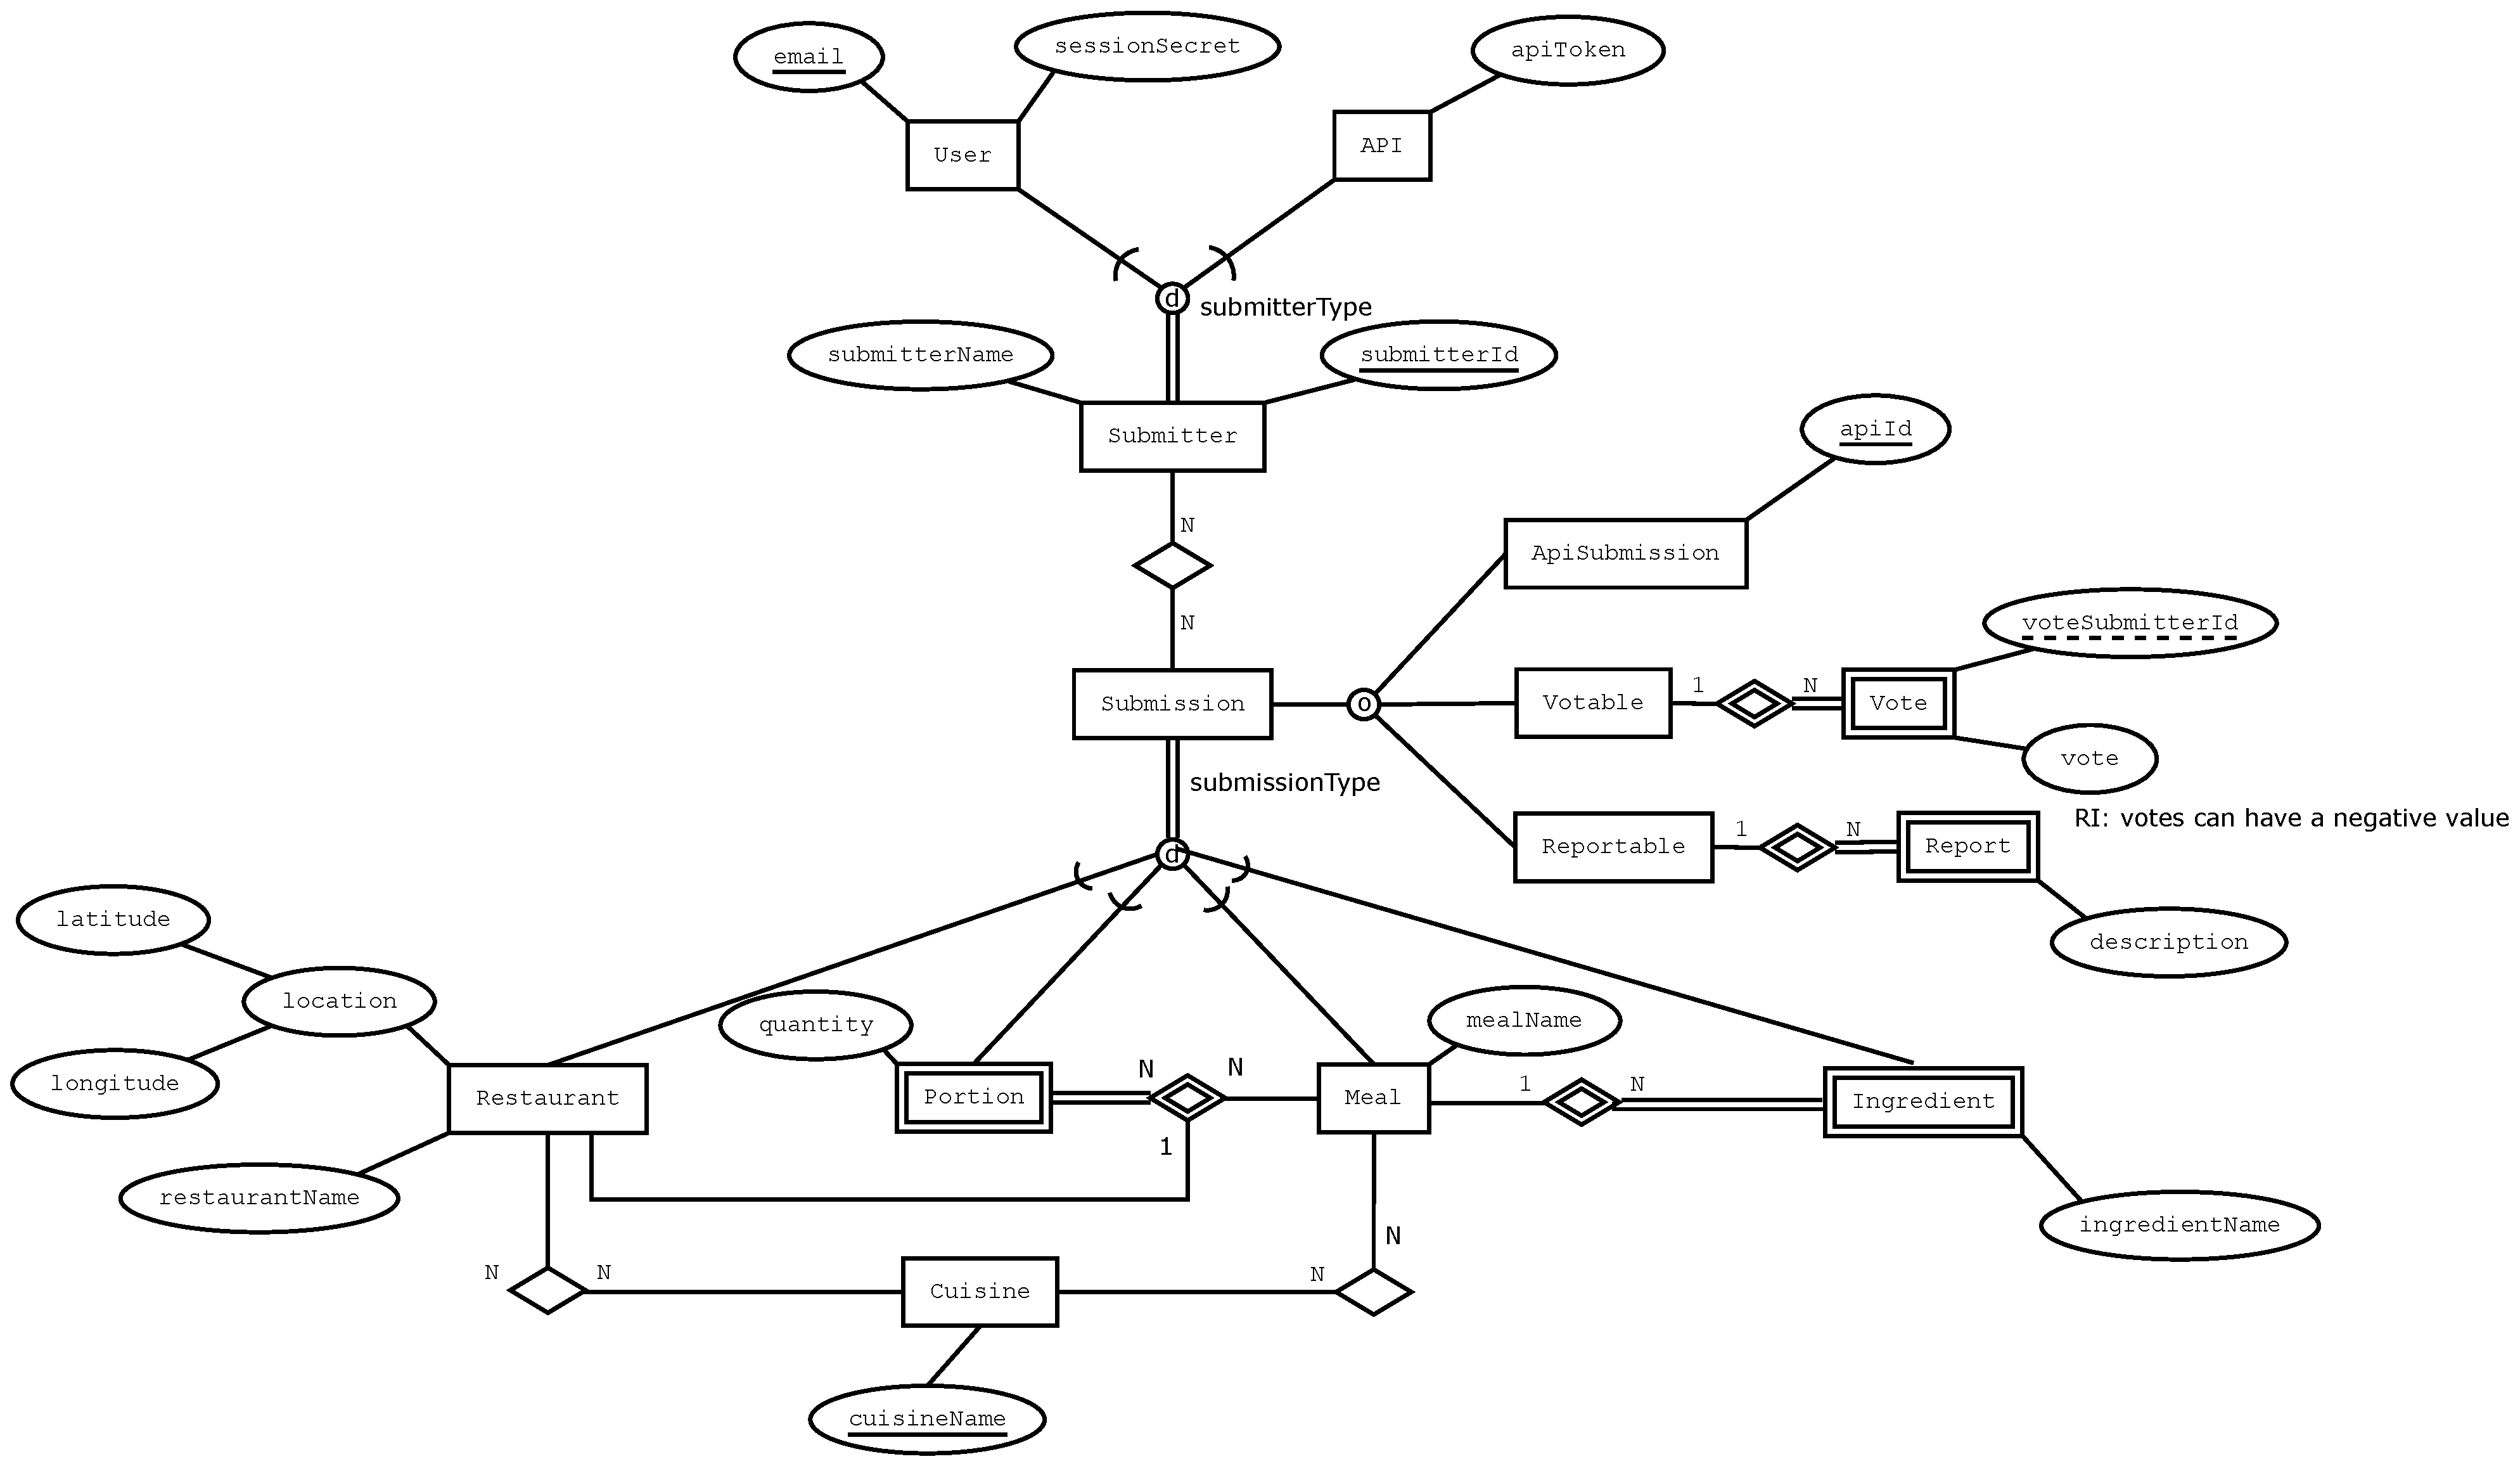
\includegraphics[scale=0.25]{_figures/Nutr.io_Database_Diagram.eps}
    \caption{Database conceptual model}
\end{figure}

\newpage
The database's relational model is present inside this report's appendix.\\

In the relational model there are tables which are not specified in the conceptual model,
those tables are a product from associations between entities, which will, not only facilitate the access queries' construction,
as provide useful data to the HTTP server's endpoints.\\

The best feature of this redesigned model is that the database can filter the user submissions from the API submissions. This is very
useful, because when the user tries to associate a meal, that does not exist in the database, to a restaurant, that is already registered
in the database, the system will have search for that meal in an external API. When the meal is found, it will be inserted in the database
as an API submission, because the data came from an external API.\\

However if another user inserts this previously inserted meal to another registered restaurant, it will insert as an user's submission, because
the data already existed in the database and the user just built the association between the specific meal and the specific restaurant.\\

This process, which resembles how memory pointers work, provides a high scalability and, cooperatively with the database normalization, lowers the memory usage.

\section{HTTP server}

As previously written in this report, the HTTP server was developed in Kotlin and Spring MVC.\\

Before starting the server's development, the group had to first define its endpoints and discuss what the client was allowed to request or receive from each one of them.
The endpoint table that defines the endpoints and their tasks can be found in the appendix.\\

After defining the endpoints, the server's development started...

\begin{itemize}
    \item hypermedia type / response type (siren and application/json)
    \item errors : application/problem+json
\end{itemize}

\section{Android application}

Being a prototype, the mobile application has only the core features to work and interact with the HTTP server.

\subsection{Layout}

The group chose to create an application that offers a simple layout to the user, providing accessible menus and a
menu drawer, which implies the use of fragments instead of activities.\\

Each fragment, that has volatile information in it (live data), has a associated view model, that preserves the data while the application is running. 
As expected, the Android app also has static fragments - fragments which do not receive live data, those do not have any view model associated.\\

Many fragment that use live data have recycler view lists, which means that for each list there's the need to have an adapter and a view holder, called by the adapter,
to bind the live data to the respective layout elements.\\

So each list that uses a diferent model class, creates its own adapter and viewholder for its specific model extending from an abstract adapter and view holder.

\subsection{HTTP requests}

The volley framework was implemented to allow the application to make asynchronous server requests.

As most of the server endpoints send responses in JSON format, the application is using the Jackson library to deserialize and serialize JSON.